\documentclass{article}
\usepackage{xeCJK}
\usepackage{graphicx}
\graphicspath{{figures/}}
\usepackage{float}
\usepackage[scale=0.8]{geometry}
\usepackage{hypertoc}
\usepackage{hyperref}
\begin{document}
	\tableofcontents
	\section{排队论基础}
	 \textbf{资源的有限性} 和\textbf{ 需求的随机性} 是 排队现象存在的基础;\\
	  由于 顾客到达 和 服务完毕的时间 都是 不确
	 定 的,绝大多数排队系统工作于 随机状态。
	 \section{排队论的概念}
	 \subsection{基本概念}
	 \subsubsection{三个参数}
	 \begin{itemize}
	 	\item  服务员数目m
	 	\item 顾客到达率 $\lambda$ ,相邻两顾客到达的时间间隔$t$,其$\textnormal{统计平均值}\overline{t}=\frac{1}{\lambda}$
	 	\item 服务员服务速率$\mu$ ,顾客服务时间$\tau$,其统计平均值为$\overline{\tau}=\frac{1}{\mu}$\begin{itemize}
	 		\item m = 1,$\mu$为服务速率
	 		\item m >1 ,$m\mu$为服务速率
	 	\end{itemize}
	 \end{itemize}
 	\subsubsection{一般性质}
 	\begin{itemize}
 		\item 平稳性,在时间间隔t内,到达 到达k 个顾客的概率只与t的长 的长
 		度 有关,而与这间隔的起始时刻无关。
 		\item 无后效性,顾客到达时刻互相独立,即顾客各自独立地
 		随机到达。
 		\item 疏稀性,在$\delta t$ 内只有一个顾客到达或没有顾客到达。
 	\end{itemize}
 	满足上三个条件的随机流成为\textbf{简单流},简单流的到达间隔是负指数分布,在一段时间内到达的顾客数服从泊松分布。
 	\subsubsection{到达时间分布}
	\begin{figure}[H]
		\centering
		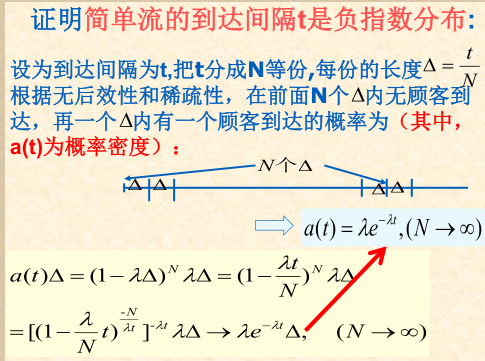
\includegraphics[width=0.5\linewidth]{figures/prove_1}
		\caption{}
		\label{fig:prove1}
	\end{figure}
	\begin{figure}[H]
		\centering
		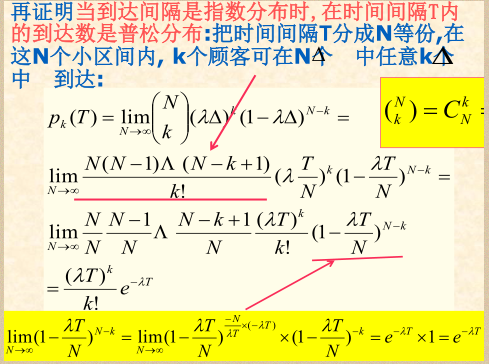
\includegraphics[width=0.5\linewidth]{figures/prove_2}
		\caption{}
		\label{fig:prove2}
	\end{figure}
	(0,t)时间内有顾客达到的概率:$p = 1- p_0(t) = 1 - e^{-\lambda t}$,即1-(0,t) 时间内没有人到达的概率
	\subsubsection{服务时间分布}
	同到达时间,只用将字母$\lambda \textnormal{换成} \mu$
	\subsubsection{排队系统表示方式}
	$A | B | m(N,n) $
	\begin{itemize}
		\item A--顾客到达时间间隔分布
		\item B--服务时间间隔分布
		\item m--窗口数
		\item N--潜在顾客数
		\item n--截止队长
	\end{itemize}
	\subsubsection{常见几种分布}
	\begin{enumerate}
		\item M分布
		\item $E_r$分布,适用于成批处理的排队。
		\item $D$分布,冲激
		\item $E_r,D$分布
		\item $H_R$分布,R阶指数分布
	\end{enumerate}
	\subsection{系统的工作方式}
	 排队系统的运行性能不仅与上述的统计分布
	有关,还与系统预先规定的 工作方式有关 。
	\begin{itemize}
		\item 排队规则 是指服务机构是否允许排队
		\item  服务规则 是指在排队等待情形下 服务的顺
		序 是什么
	\end{itemize}
	\subsubsection{排队规则}
	\begin{figure}[H]
		\centering
		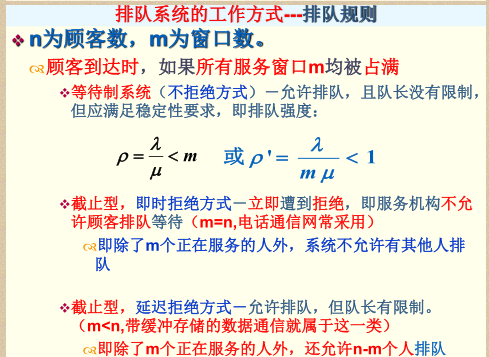
\includegraphics[width=0.5\linewidth]{figures/prove_3}
		\caption{}
		\label{fig:prove3}
	\end{figure}
	\subsubsection{服务规则}
	\begin{itemize}
		\item 先到先服务
		\item 后到先服务
		\item 优先制服务
		\item 随机服务
	\end{itemize}
	\subsection{主要性能指标}
	\begin{figure}[H]
		\centering
		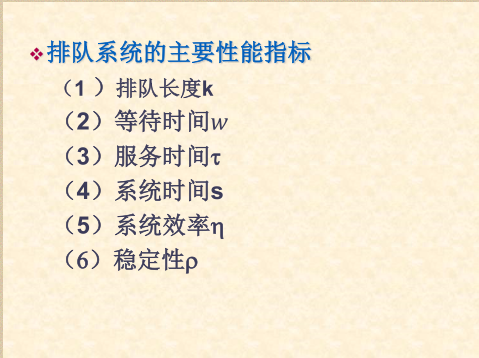
\includegraphics[width=0.5\linewidth]{figures/prove_4}
		\caption{}
		\label{fig:prove4}
	\end{figure}
	\subsection{M|M|1问题}
	求解步骤:
	\begin{enumerate}
		\item 确定状态变量
		\item 画出状态转移图
		\item 列出状态转移方程
		\item 求解状态转移方程
	\end{enumerate}
	\subsubsection{M|M|1 参数求解}
	\begin{figure}[H]
		\centering
		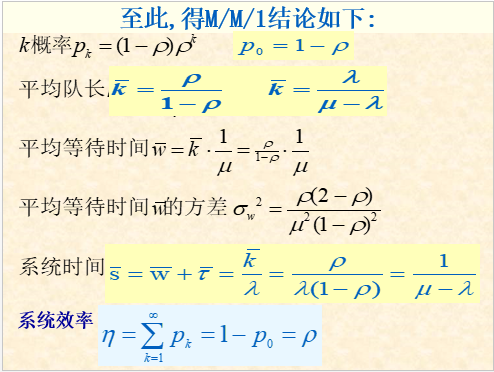
\includegraphics[width=0.5\linewidth]{figures/prove_5}
		\caption{}
		\label{fig:prove5}
	\end{figure}
	\subsubsection{M|M|1 闲期和忙期}
	\begin{figure}[H]
		\centering
		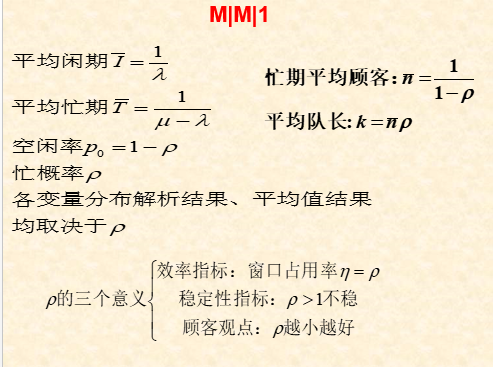
\includegraphics[width=0.5\linewidth]{figures/prove_6}
		\caption{}
		\label{fig:prove6}
	\end{figure}
	\subsubsection{通信网中的排队论计算}
	\textbf{计算通信网中的M/M/1系统指标,将原来的$\mu$ 换为$\mu C$}
	\subsection{M|M|m(n)}
	压缩排队长度的措施:
	\begin{itemize}
		\item 增加窗口数
		\item 截止排队长度
	\end{itemize}
	融合上述两种方式,成为\textbf{截止型多窗口排队系统}
	 \textbf{即时拒绝系统的拒绝概率(爱尔兰公式)}
	 \[
	 	p_n = \frac{a^m/{m!}}{\sum_{r=0}^{m}a^r/{r!}}
	 \]
	 \subsubsection{业务量和呼叫量}
	 业务量是在\textbf{指定时间内线路被占用的总时间}\\
	 呼叫量定义为\textbf{线路占用时间和观察时间之比}。
	 
	 \section{通信网络的业务模型与分析}
	 \subsection{阻塞率和呼损率}
	 拒绝状态站全部状态的百分比。
	 \subsubsection{时间阻塞率}
		\[
			p_n = \frac{\textnormal {阻塞时间}}{\textnormal {总观察时间}}
		\]
	\subsubsection{呼叫阻塞率}
	\begin{displaymath}
		p_c = \frac{\textnormal {被拒绝的呼叫次数}}{\textnormal {总呼叫次数}}
	\end{displaymath}
	总有:$p_c \le p_n$。因为$p_c$只在呼叫的时候统计,但在不呼叫的时候也可能发生呼损。
	\subsection{用户数为有限制N的准随机呼叫}
	\[
		p_c = \frac{(N-n)\lambda p_n}{\sum_{r=0}^{n}(N-r)\lambda p_r}
	\]
	N为潜在用户数,n为截止队长。特别地,当$\lambda --> \inf$时,
	\[
		p_c = \frac{\lambda p_n}{\sum_{r=0}^{n}\lambda p_r}
	\]
	
	\subsection{业务分析}
	线路利用率:\( \sum_{r=1}^{m}\frac{1}{r}P_r  \),其中,m为该系统服务台(维数),$P_r$为r状态的概率
	\subsubsection{即时拒绝系统}
	\begin{figure}[H]
		\centering
		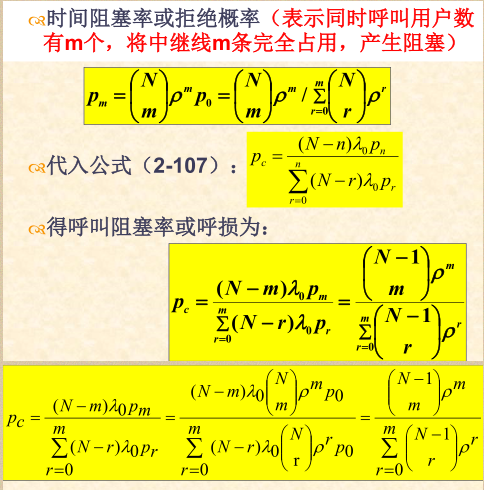
\includegraphics[width=0.5\linewidth]{figures/prove_7}
		\caption{}
		\label{fig:prove7}
	\end{figure}
	\subsubsection{主备线即时拒绝系统}
	\begin{figure}[H]
		\centering	
			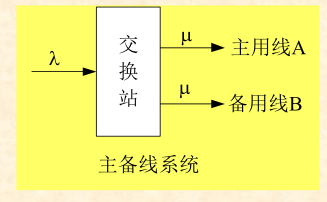
\includegraphics[width=0.4\linewidth]{figures/prove_12}
			\\	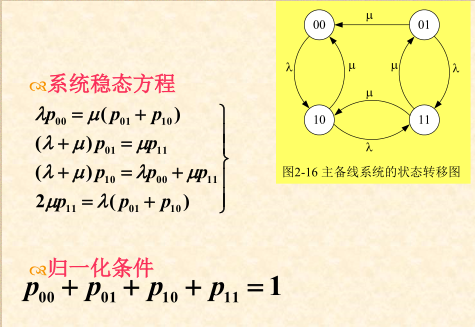
\includegraphics[width=0.5\linewidth]{figures/prove_8}
	
		\caption{}
		\label{fig:prove8}
	\end{figure}
	\subsubsection{公用备线即时拒绝系统}
	\begin{figure}[H]
		\centering
		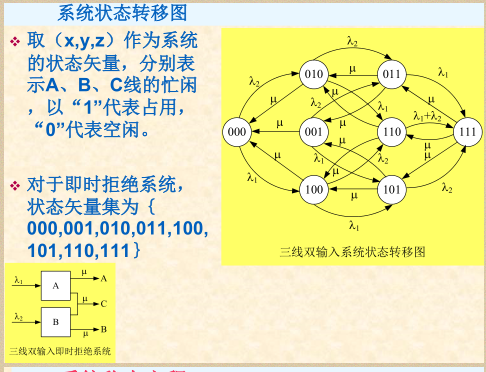
\includegraphics[width=0.5\linewidth]{figures/prove_9}
		\caption{}
		\label{fig:prove9}
	\end{figure}
	公用备线系统与主备线系统的比较:
	公用备线系统减少一条信道,其信道利用率提高,但是呼损率有损增加。在业务量不太大的情况下,采用公用备线是很合算的。
	\subsubsection{优先制排队系统}
	\begin{figure}[H]
		\centering
		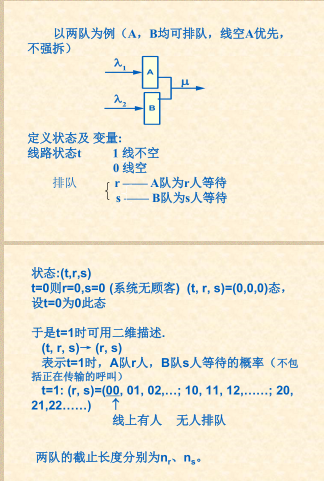
\includegraphics[width=0.5\linewidth]{figures/prove_10}
		\caption{}
		\label{fig:prove10}
	\end{figure}
	\begin{figure}[H]
		\centering
		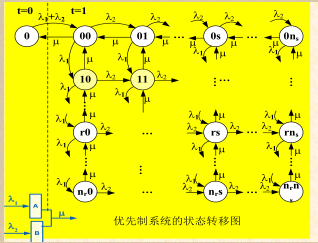
\includegraphics[width=0.5\linewidth]{figures/prove_11}
		\caption{}
		\label{fig:prove11}
	\end{figure}
	
\end{document}